\documentclass[a4paper,11.5pt]{article}
\usepackage[latin1]{inputenc}
\usepackage[T1]{fontenc}
\usepackage[english]{babel}
\usepackage{graphicx}
\usepackage{amsmath}
\usepackage{amsfonts}
\usepackage{multirow}
\usepackage{booktabs}
\usepackage{bbold}
\usepackage{mathtools}
\usepackage{mathrsfs}
\usepackage{enumitem}
\usepackage{array}

\setlength{\parindent}{0pt}
\DeclarePairedDelimiter{\floor}{\lfloor}{\rfloor}
\DeclarePairedDelimiter{\ceil}{\lceil}{\rceil}

\newcommand{\vt}{\boldsymbol}

\title{Digital Communications - HW3}
\author{Jacopo Pegoraro, Edoardo Vanin}
\date{21/05/2018}

\begin{document}

\maketitle

\section*{Problem}

We have to implement six different versions of the receiver structure in a QPSK modulation scheme. First we present the setup of the transmitter and the channel as given, the we analyze the different configurations one by one and give a brief discussions of the resulting probabilities of symbol error obtained from simulation over different values of the SNR at the channel output, $\Gamma$. 

\section*{Transmitter and Channel}

The system takes a sequence of input symbols $a_k$ at sampling time $T=1$ and applies an upsampling of factor 4, obtaining $a_k'$ at $T/4$. This new sequence is then filtered by $q_c$ as described by the following difference equation:
\begin{equation}
s_c(nT/4) = 0.67 s_c((n-1)T/4) + 0.7424 a_{n-5}
\end{equation}
After the filtering white noise is added. The SNR at the channel output for all the configurations in this first phase is $\Gamma = 10$ dB, so from the following relations we can derive $\sigma_w^2$, the variance of the complex valued Gaussian noise:
\begin{equation}
\Gamma = \frac{M_{s_c}}{N_0\frac{1}{T}} = \frac{\sigma_a^2 E_{q_c}}{\sigma_w^2} \longrightarrow \sigma_w^2 = \frac{\sigma_a^2 E_{q_c}}{\Gamma} = 2\sigma_I^2
\end{equation}
where $\sigma_I^2$ is the variance per component. In addition we can also compute the PSD as $N_0=\sigma_w^2 T_c=\sigma_w^2/4$, because the sampling time $T_c$ at which we add the noise is $T/4$.
In figure \ref{fig:qc} we plot the impulse response and the frequency response of the filter $q_c$.
This implementation of the transmitter is the same for all the following discussion.

\begin{figure}[ht]
	\begin{center}   
		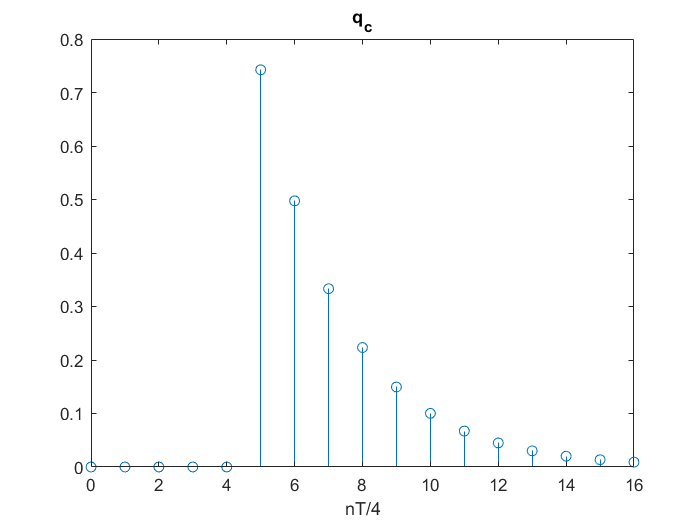
\includegraphics[width=9cm]{figs/q_c.png} 
		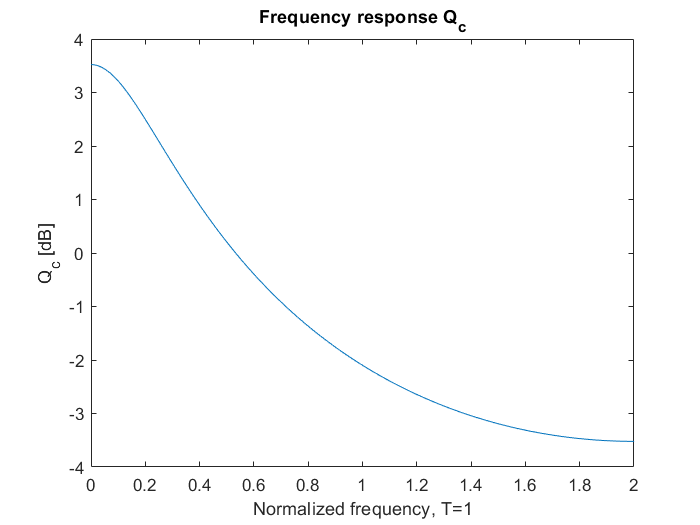
\includegraphics[width=9cm]{figs/Qc.png} 
		\caption{Impulse and frequency response of the filter $q_c$ at $T/4$.}
		\label{fig:qc}
	\end{center}
\end{figure} 



\section*{Point A}


\begin{figure}[ht]
	\begin{center}   
		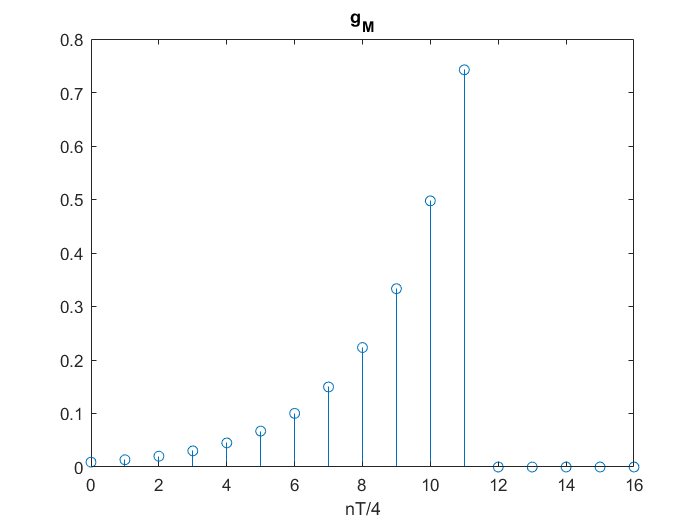
\includegraphics[width=\textwidth]{figs/A_gm.png} 
		\caption{Impulse response of the matched filter $g_{M}$ for the receiver in point A.}
		\label{fig:A_gm}
	\end{center}
\end{figure} 

\begin{figure}[ht]
	\begin{center}   
		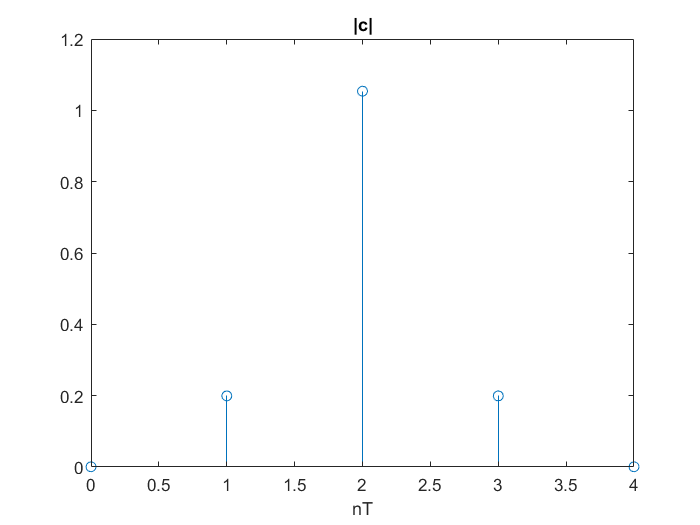
\includegraphics[width=\textwidth]{figs/A_c.png} 
		\caption{Magnitude of the impulse response of filter $c$ in point A.}
		\label{fig:A_c}
	\end{center}
\end{figure}

\begin{figure}[ht]
	\begin{center}   
		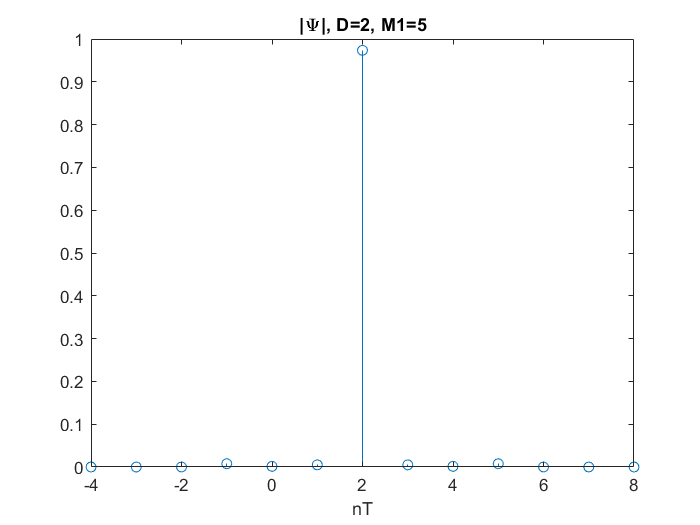
\includegraphics[width=\textwidth]{figs/A_psi.png} 
		\caption{Magnitude of the impulse response of the system $\psi$ in point A.}
		\label{fig:A_psi}
	\end{center}
\end{figure}



\section*{Point B}

\begin{figure}[ht]
	\begin{center}   
		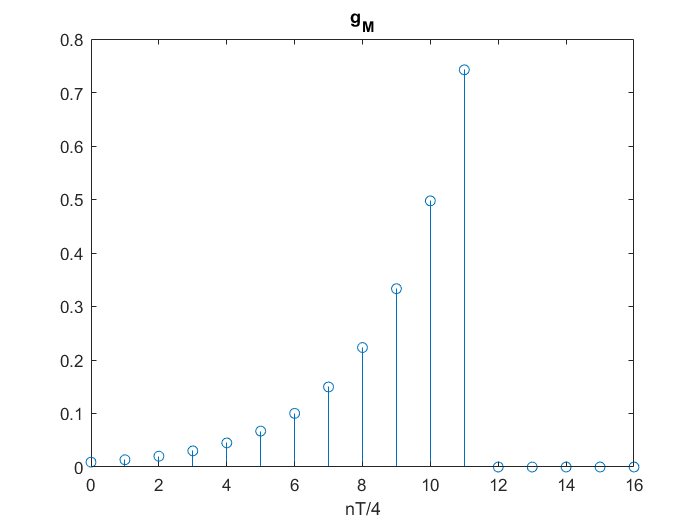
\includegraphics[width=\textwidth]{figs/B_gm.png} 
		\caption{Impulse response of the matched filter $g_{M}$ for the receiver in point B.}
		\label{fig:B_gm}
	\end{center}
\end{figure}

\begin{figure}[ht]
	\begin{center}   
		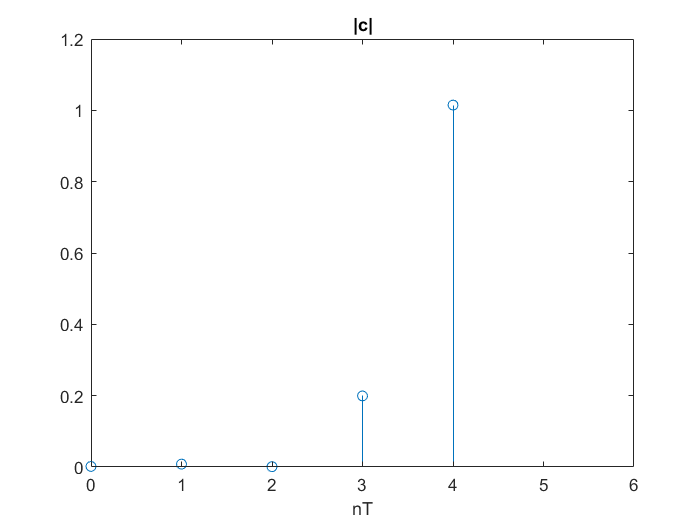
\includegraphics[width=\textwidth]{figs/B_c.png} 
		\caption{Magnitude of the impulse response of the filter $c$ (feedforward filter) for the receiver in point B.}
		\label{fig:B_c}
	\end{center}
\end{figure}

\begin{figure}[ht]
	\begin{center}   
		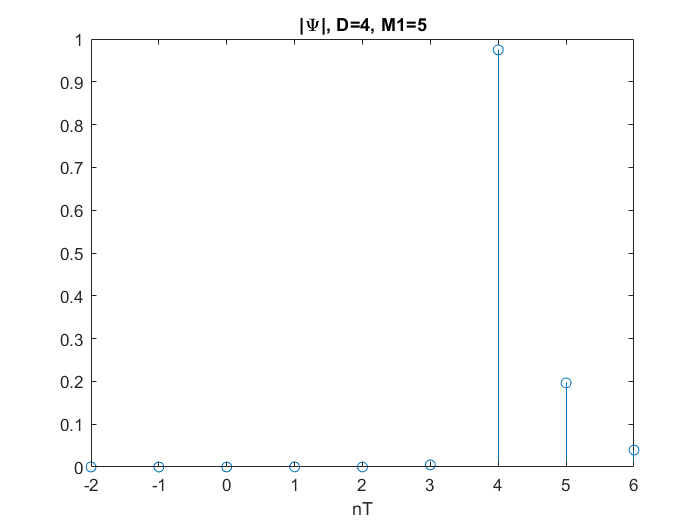
\includegraphics[width=\textwidth]{figs/B_psi.png} 
		\caption{Magnitude of the impulse response of the system $\psi$ in point B.}
		\label{fig:B_psi}
	\end{center}
\end{figure}

\begin{figure}[ht]
	\begin{center}   
		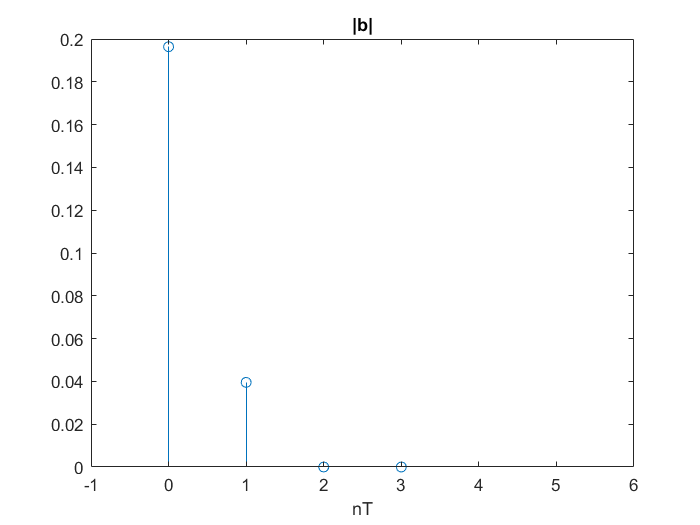
\includegraphics[width=\textwidth]{figs/B_b.png} 
		\caption{Magnitude of the impulse response of the filter $b$ (feedback filter) in point B.}
		\label{fig:B_b}
	\end{center}
\end{figure}

\section*{Point C}

\section*{Point D}

\section*{Point E}

\section*{Point F}

\section*{Simulation results}

\begin{figure}[ht]
	\begin{center}   
		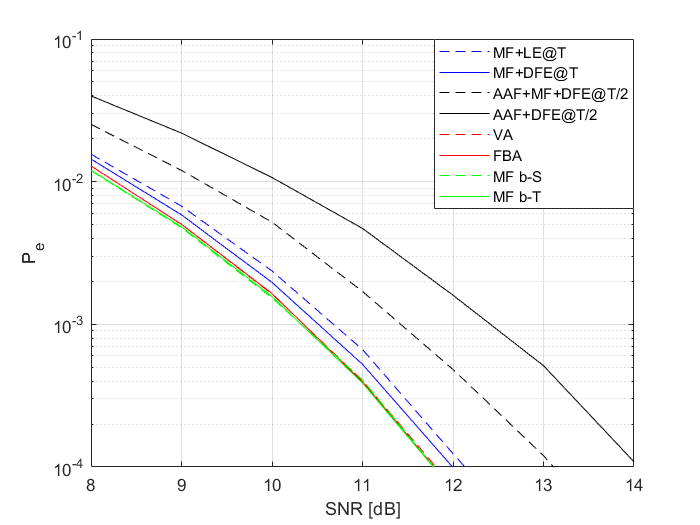
\includegraphics[width=\textwidth]{figs/SNR_Pe.png} 
		\caption{Results of the simulation over values of the SNR at the channel output from 8 dB to 14 dB.}
		\label{fig:B_b}
	\end{center}
\end{figure}


\begin{table}[htbp]
	\begin{center}
		\begin{tabular}{p{2.7cm}ccc}
			\toprule
			
			$nT_y$ & $h$ & $\hat{h}_{corr}$ & $\hat{h}_{ls}$\\
			\midrule
			0 & 1.0000  & 1.0054 & 0.9991  \\
			1 & 0.9635 & 0.9247 & 0.9613  \\
			2 & 0.4641 & 0.5002 & 0.5062 \\
			3 & -0.0001 & 0.0202 & 0.0255  \\
			4 & -0.2155 & -0.2549 & -0.2253\\
			\midrule
			%& \multicolumn{3}{c}{} \\
			& Real & Corr & LS \\
		    \cmidrule(lr){2-4}
		    $\sigma_w^2$ [dB] & -8 & -7.9776 & -8.0404  \\
			\bottomrule
		\end{tabular}
	\end{center}
	\label{tab:}
	\caption{.}
\end{table} 
 




\begin{thebibliography}{15}
	
	\bibitem{nevio<3}
	Nevio Benvenuto, Giovanni Cherubini,
	\textit{Algorithms for Communication Systems and their Applications}. 
	Wiley, 2002.
	

	
\end{thebibliography}

\end{document}